\question{Аберрации электронных линз}

Теория тонких линз основана на паре приближений:
\begin{itemize}
  \item в выражении для потенциала \eqref{eq08.2.15} оставляются только два
    первых слагаемых,
  \item параксиальное приближение.
\end{itemize}

Поэтому, при конструировании реальных электронных устройств, в последних
наблюдаются отклонения траекторий от теоретических. Такие отклонения называют
аберрациями.

\subquestion{Хроматическая аберрация}

В электронно-оптических системах под хроматической аберрацией понимают ошибки
изображения, обусловленные разбросом начальных скоростей падающих на линзу
электронов.

Быстрые электроны находятся в пространстве взаимодействия меньше, чем медленные,
следовательно, для быстрых и для медленных электронов у линзы будет разные
фокусные расстояния (рис.~\pic{16chrome}), и каждая точка объекта на изображении
будет размыта в пятно.

\begin{figure}[h!]
  \center
%  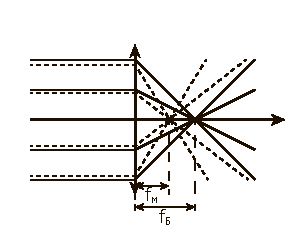
\includegraphics[width=.3\textwidth]{16_chromatic} \hspace{1em}
%  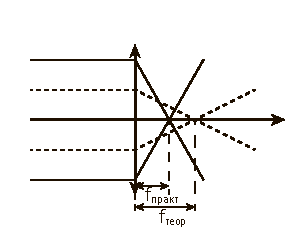
\includegraphics[width=.3\textwidth]{16_spherical} \\
  \parbox{.3\textwidth}{\caption{Схематичное изображение хроматической
    аберрации} \label{pic16chrome}} \hspace{1em}
  \parbox{.3\textwidth}{\caption{Схематичное изображение сферической
    аберрации} \label{pic16sphere}}
\end{figure}

\subquestion{Сферическая аберрация}

Сферическая аберрация является результатом проявления нелинейной зависимости
преломляющей силы линзы от радиальной координаты (рис.~\pic{16sphere}.

Данный вид аберрации проявляется при фокусировке широких пучков, то есть
нарушается условие параксиальности.

\subquestion{Аберрации косых пучков}

Если объект достаточно велик, то некоторые его точки будут удалены настолько,
что при создании его изображения будут участвовать электроны, траектории которых
сильно наклонены к оси симметрии~-- т.~н. косые пучки.
\begin{figure}[h!]
  \center
%  \includegraphics[width=.6\textwidth]{16_skew_beam} \\
  \caption{Виды аберрации косых пучков: а~-- кома, б~-- астигматизм, в~--
    дисторсия}
  \label{pic16skew}
\end{figure}

В результате изображение предмета на краях становится размытым: кома,
астигматизм\\ (рис.~\pic{16skew}: а, б); или изображение будет в искаженном
масштабе: подушечная (рис.~\pic{16skew}: в\( _1 \)) и бочкообразная
(рис.~\pic{16skew}: в\( _2 \)) виды дисторсии.

Такие аберрации возникают из-за большого угла наклона траекторий электронов к
оси~-- нарушается параксиальное приближение.
